The results consist of three main parts:
\begin{itemize}
\item A benchmark of the impact of different parameters on the
  tracking performance, performed on synthetic videos and evaluated
  programmatically
\item Test runs on real data with the best performing parameters from
  the benchmark, evaluated manually
\item Conclusions concerning the feasibility of a probabilistic
  whisker tracking system.
\end{itemize}

\section{Parameter Benchmark}

A benchmark was performed in order to identify how tracking
performance is affected by the different parameters. The benchmark was
performed on generated videos of synthetic whiskers, which enabled
programmatic evaluation of the results since the correct shapes of the
whiskers, the \emph{ground truth}, were known.

\subsection{Test data}
\label{sec:test-data}

The test data consisted of a single generated video of synthetic
whiskers. The video contained 6 whiskers and was 64 frames long. Each
whisker had length 200 and a random base shape $\Spline{\omega}$, with
$a_3, a_2, a_1$. Each $a_i$ was in the range $\left[0,
  \sigma_i\right)$, where $\sigma_3 = 1.6 \cdot 10^{-5}, \sigma_2 =
4\cdot 10^{-3}, \sigma_1 = 1$. Each whisker was then assigned a random
phase $d \in \left[0, 2\pi\right)$, and the shape at time step $t$ was
$\left(\Spline{\omega}\right) \sin(\frac{2\pi t}{30} + d)$.

The shape and the frequency $\frac{1}{30}$ were selected through
manual inspection of a video of real whiskers in order to make the
generated whiskers roughly realistic. The resulting whiskers were
roughly reminiscent of real whiskers, and 6 sample frames can be seen
in figure \ref{fig:benchmark-video}.

The database was generated with the same settings as the video, and
contained $2^{14} = 16384$ transitions. Each transition consisted of a
``from'' part $\tf$ and a ``to'' part $\tt$. $\tf$ was created by
generating a base state and phase in the same way as for the video,
and setting $t=0$. $\tt$ was created by taking $\tf$ and increasing
the phase by $\frac{2\pi}{30}$.

\begin{figure}
  \centering
  \begin{tabular}{ccc}
    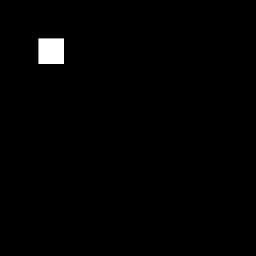
\includegraphics[width=0.3\textwidth]{benchmark-video/frame-00000.png} &
    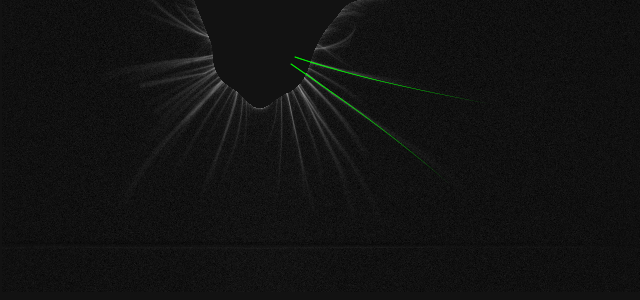
\includegraphics[width=0.3\textwidth]{benchmark-video/frame-00005.png} &
    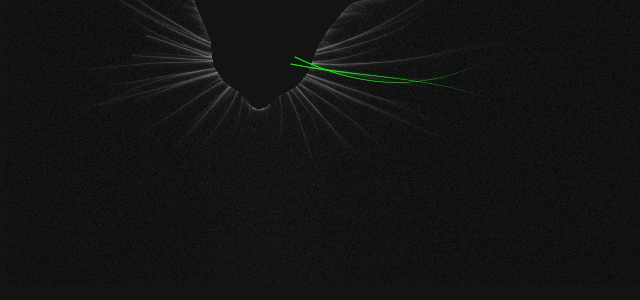
\includegraphics[width=0.3\textwidth]{benchmark-video/frame-00010.png}\\
    Frame 0 & Frame 5 & Frame 10\\
    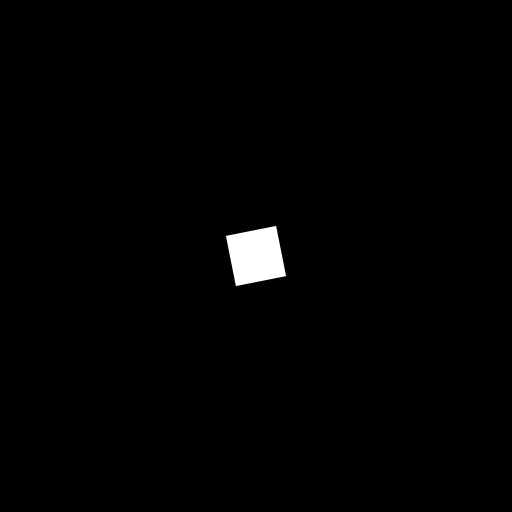
\includegraphics[width=0.3\textwidth]{benchmark-video/frame-00015.png} &
    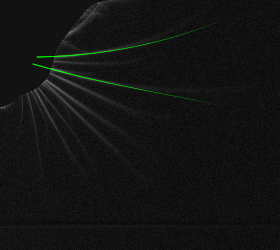
\includegraphics[width=0.3\textwidth]{benchmark-video/frame-00020.png} &
    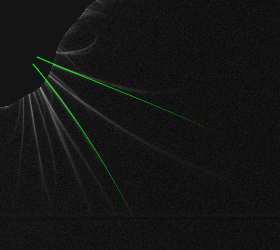
\includegraphics[width=0.3\textwidth]{benchmark-video/frame-00025.png}\\
    Frame 15 & Frame 20 & Frame 25
  \end{tabular}
  \caption{Sample frames from the testing video.}
  \label{fig:benchmark-video}
\end{figure}  


\subsection{Evaluated parameters}
The following parameters were evaluated:

\begin{description}
\item[n] Number of particles
\item[p] In which $\Lp$ space to compute $\Lpnorm{\tf - x_{t-1}}$ in
  the prediction step
\item[a] The exponent for the weights in the prediction step, $w =
  \Lpnorm{\tf - x_{t-1}}^{-a}$
\item[$\sigma$] Standard deviation modifier for the offset in the
  prediction step. Standard deviations for the $\omega^3, \omega^2$
  and $\omega$ terms are $\sigma\sigma_3, \sigma\sigma_2$ and
  $\sigma\sigma_1$, respectively.\footnote{See section
    \ref{sec:test-data} for the $\sigma_i$ values.}
\item[g] The exponent for the importance in the filtering step
\end{description}

Table \ref{tbl:testcases} shows the tested values.

\begin{table}
  \centering
  \begin{tabular}{c|l}
    Parameter & Values\\
    \hline
    $n$ & 64, 128, 256, 512\\
    $p$ & 2, 4, 8\\
    $a$ & 1, 2, 4, 8\\
    $\sigma$ & 0.025, 0.05, 0.1, 0.2\\
    $g$ & 1, 2, 4, 8
  \end{tabular}
  \caption{Specification of test cases.}
  \label{tbl:testcases}
\end{table}

\subsection{Benchmark procedure}

The benchmark was run on the test video for each combination of
parameters in table \ref{tbl:testcases}. The output from the benchmark
is an error matrix $\epsilon_{i,t}$, where index $i, t$ contains
$\Lpnorm[2]{Z_t - x_t}$, the $\Lp[2]$ distance between the ground
truth and estimated shape for whisker $i$ at time $t$. From this a
list $\epsilon_i$ was computed as the root mean square of
$\epsilon_{i,t}$ in the $t$ direction. Finally, the maximum value in
$\epsilon_i$ was selected as the \emph{error} $\epsilon$ of that
run. This gives us the error tensor

\begin{equation}
  E_{n,p,a,\sigma,g} = \argmax{i} \sqrt{\left(\sum\limits_t
      \epsilon_{i,t}^2 \right)} ~ \forall \left(n, p,
    a, \sigma, g\right).
\end{equation}

Note that the absolute magnitude of the error $\epsilon$ is irrelevant
- it is the ratios between these errors that is interesting. One could
argue for instead using the relative error $\Lpnorm[2]{Z_t - x_t} /
\Lpnorm[2]{Z_t}$, but the relative error is misleading here. The
reason is that a deviation from a very bent whisker would then be
considered better than the same deviation from a very straight
whisker. Therefore the absolute error is used for the analysis.

The measures that will be used as fitness of the parameters:
    \begin{description}
        \item[$\int{||\epsilon(t)||_{L^p}}dt$]
            integrating over time the the difference
            with the ground truth (do this for L{1:10} and see if it correlates with
            the p choosed (to see how much it deviates from the ground truth)
        \item[$\int{\Response{x_t}{I_t}{\phi} }dt$] 
            integrating over time the response
            for the choosed hypothesis (to see how the different image transformation
            affects the results, that is if it only follows what it thinks is best
            (phi))
        \item[Subjective] 4 image samples
    \end{description}
And all this are done for all 4 benchmark videos.

<<more shall come>>

%"There are many metrics by which a model may be assessed." - Encyclopedia

%Tillvägagångsätt:
%1. Since we have prior knowledge about the effect off varying the parameters n,N
%they will firstly be set to a sufficently large value.
%2. A partion of the test-matrix will then be evaluated by ... parameter group 
